\thesischapterexordium

\section{脑电的产生、现状和诊断学应用}
脑电的先驱人物,英国人Richard Caton (1842-1926)在1875-1887年间先后在动物上开展研究\citing{haas2003hans}。他把两个单极电极放在动物大脑的左右半球上,或者是把一个电极放在在皮层或灰质另一个电极放在颅骨表面,记录到了电流,并发现这些电流随着睡眠增强并呈现出与心跳、呼吸节律无关的变化,这些电流容易受到缺氧或麻醉状态的影响,最终随着动物的死亡消失。

基于Richard Caton的工作,德国人Hans Berger (1873-1941) 1924年在对一位17岁男孩进行外科手术时第一次记录到了人类脑电,
经过五年的反复推敲,于1929年正式了发表题为Über das Elektrenkephalogramm des Menschen (人类的脑电) \citing{berger_uber_1929,tudor2005hans}的文章,他称“第一次从人头皮表面记录到了人脑电活动”。 一段早期记录的脑电波如图\ref{fig1}所示。 在文章中,他也首次描述了脑电的$\alpha$和$\beta$波,并注意到脑电随着注意和情感效应而变化,最早的$\alpha$波又称为Berger波。
Berger也首次描述了在癫痫等脑疾病中脑电波特征有变化的现象。
\begin{figure}
	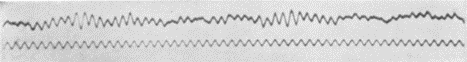
\includegraphics[width=15cm]{pic/xulun/EEGwave.png}
	\caption{Berger记录的第一条脑电波,引自文献\citing{berger_uber_1929}}
	\label{fig1}
\end{figure}

今天,人们对脑电的定义更加清楚,脑电来自于突触后电位的同步活动,如图\ref{fig2}\citing{lopez2014dry}被头表电极经差分记录放大得到,放映了神经源的有节律的震荡\citing{niedermeyer_electroencephalography_2005}。
\begin{figure}
	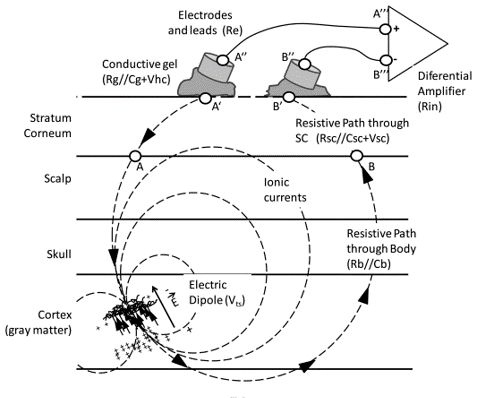
\includegraphics[width=12cm]{pic/xulun/EEGrecord.png}
	\caption{脑电产生的偶极子、电流与差分记录,引用自文献\citing{lopez2014dry}}
	\label{fig2}
\end{figure}
在$\alpha$和$\beta$节律的基础上,人们根据脑电的时域信号的频率幅度特性变化,将脑电分为如图\ref{fig3}五种不同类型的波,包括$\delta$节律(<4Hz)、$\theta$节律(4-7Hz)、$\alpha$节律(8-15Hz)、$\beta$节律(16-31Hz)和$\gamma$节律(>32Hz),根据频率不同的特点不同的节律也称为不同的频带。 这些节律随着频率增加,大致呈现幅度下降的特点,与大脑的认知过程状态、神经功能
生长发育成熟或老化息息相关。
\begin{figure}
	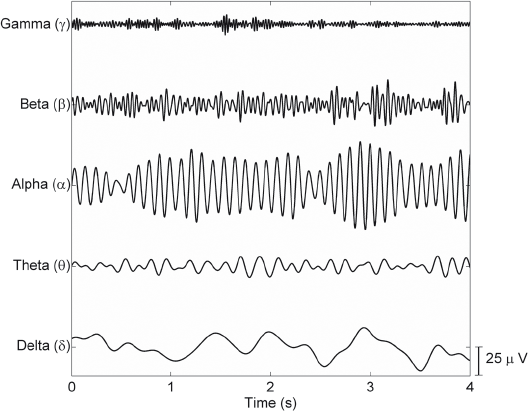
\includegraphics[width=12cm]{pic/xulun/EEGrhythm.png}
	\caption{脑电的不同节律波形特点,引用自文献\citing{campisi2012eeg}}
	\label{fig3}
\end{figure}

脑电在诊断方面的应用主要指的是时间诱发电位(Event related potentials)或者脑电的谱分析,前者指的是被试对某种刺激产生的锁时的脑电波动,后者指的是对代表神经震荡的脑电波信号进行的频谱分析。因为癫痫会引起脑电记录的异常,脑电常用来诊断癫痫\citing{tatum2014handbook},也用来诊断睡眠紊乱、麻醉程度、昏迷、脑死亡、中风、肿瘤等\citing{chernecky2012laboratory}。

\section{脑电研究方法}
随着采集技术、计算机技术和信号分析方法的发展,脑电经历了产生,发展和广泛应用的阶段。 如图\ref{fig4},脑电研究方法的四个阶段可分为:早期基于拍照成像的视觉分析,对打印成纸质脑电波进行统计分析、磁盘存储的编程分析和云端存储的高性能计算分析。其中在1977-1980年,ER John提出了定量脑电概念\citing{john1977neurometrics,john1980developmental}。根据脑电分析方法类型,分为标准
化去伪差、头表源空间、时空频、谱网络、线性非线性、回归分类预测等。 其中的标准化指的是对数据存储格式和脑电的参考进行标准化,去伪差指的是对各种各样的伪迹信号(比如眼电、心电、肌电、电极接触不良、工频干扰等)利用独立成分分析等方法进行伪迹去除;按照分析的空间可以分为头表空间的多通道电极信号的分析和通过源定位技术\citing{rd_pascual-marqui_review_1999}进行溯源在源空间的分析;按照分析的角度可以分为脑电波时域波形幅度等特点、电极或者源上的空间域分析和通过傅里叶变换对信号的时不变特征进行的频域谱分析;根据是否关注信号之间的联系又可以分为谱分析和一般基于图论的对脑连接特征进行网络分析;按照对脑电信号分析的复杂程度,可以分为简单的线性比如基于高斯稳态信号的统计分析和复杂的非线性比如复杂度、更高阶谱或者混沌动力学、熵等非稳态非随机信号分析;最后根据应用,借助于机器学习方法,可以分为脑电常模的回归和对脑状态脑疾病的分类预测等。脑电分析方法在多模态融合、心理学、脑疾病和脑
机接口、测谎等工程领域得到不同应用。
\begin{figure}
	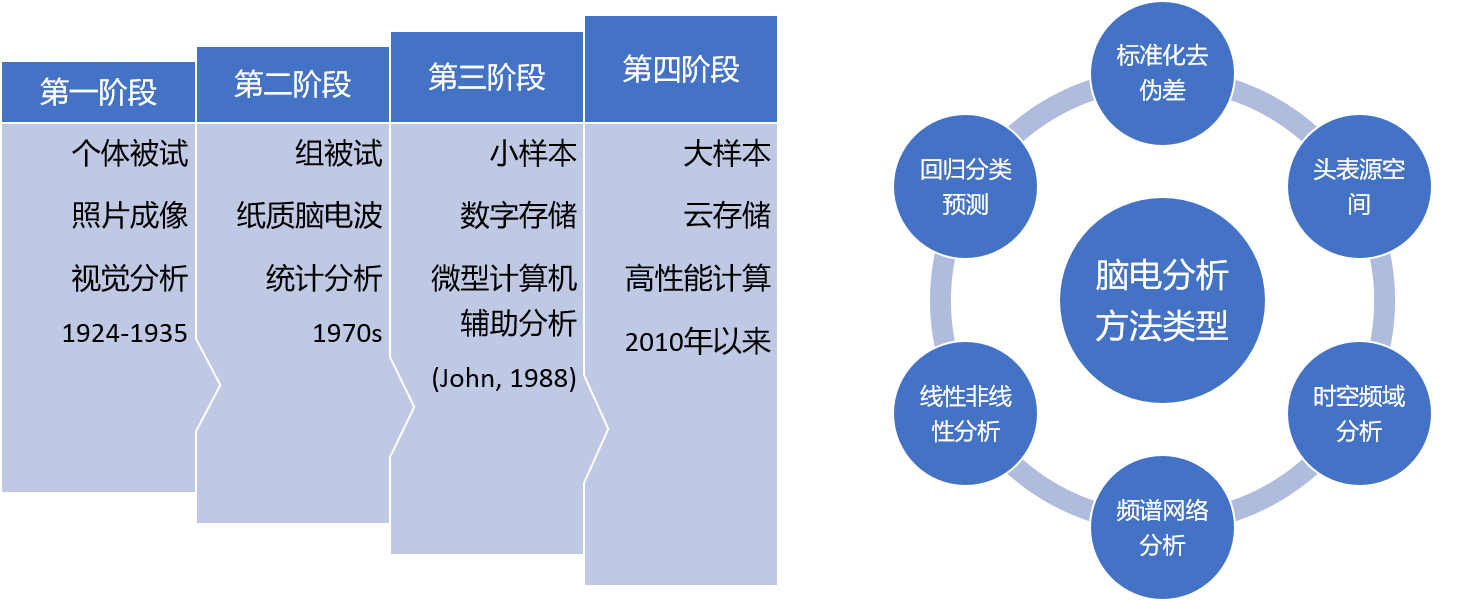
\includegraphics[width=15cm]{pic/xulun/evolution.png}
	\caption{脑电研究方法:进展和类型}
	\label{fig4}
\end{figure}

针对与本论文中密切相关的参考问题、模型选择、伪迹去除、谱分析、回归、震荡节律分析,我们接下来分节介绍。
\subsection{参考问题}
从图\ref{fig2}可知,脑电信号是活跃电极和参考电极的信号经差分放大记录得到的。 因此,脑电信号实际上是活跃电极减去参考电极得到的电位差,或电势差\citing{Fundamentals of {EEG} measurement}。根据电荷、偶极子及电场理论,测量电势的最优物理参考是位于离测量带电荷无穷远处的零电势点,这个电势点称为无穷远参考(Infinity Reference(IR))点。然而,这种理论最优的无穷远参考在实际中是不存在的,这是因为人体表面并不存在不活跃的零电位点,位于头表之外体表上的电极也会采集到心电、肌电等伪差信号,置于体外的参考电极会引入更多的环境噪声干扰。 

自脑电产生以来,人们一直在不断探究希望希望找到一种合理的参考方式采集到更加准确的脑电电位,如图\ref{fig5}所示,这包括连接耳参考\citing{garneski_t_m_and_steelman_h_f_equalizing_1958}(Linked Mastoids(LM))、平均参考\citing{offner_eeg_1950,goldman_clinical_1950}(Average Reference(AR))、左耳、右耳、偏侧耳(Ipsilateral ear)、头表电极Cz、横向双极参考、纵向单极参考等。与无穷远参考等单极参考不同,双极参考的目的是记录到局部相邻电极的相对电位,偏侧耳是一侧半球上的电极参考到这一侧的耳垂处的电极以消除左右半球的不对称性,这种双极参考记录增加了电极间差异的不确定性,采用的紧邻电极相对电位是不同于单极参考脑电电位的物理度量,在本文中我们主要研究单极参考。 其中考虑到较好的接触,Cz作为一种常见的在线记录参考;根据左右耳电位的均值为零的假设,连接耳也被广泛采用;当偶极子在匀质且各向同性传导的容积导体内,容积导体表面上的电位积分为零,我们将头看成是封闭的表面,当头表被足够多的电极均匀地分布采样并尽可能宽广地覆盖,电极上电位的均值接近于零,平均参考似乎具有接近实际的物理假设\citing{bertrand_theoretical_1985,nunez_p_l_eeg_1997,
nunez_electric_2006}。

\begin{figure}
	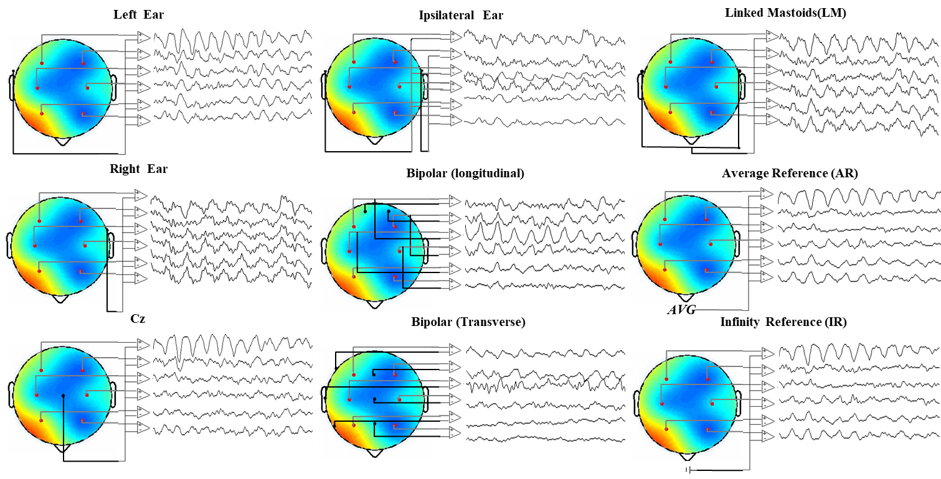
\includegraphics[width=15cm]{pic/xulun/EEGref.png}
	\caption{不统一的参考电极选择。左列为常用的单极参考,中间列为双极参考,右列为重参考。}
	\label{fig5}
\end{figure}

近年来,\cite{yao_method_2001}基于等效源技术和三层球头模型提出了参考电极标准化技术(Reference Electrode Standardization Technique, REST, 也称为零参考)。 零参考是一种离线重参考,利用等效源作为桥梁可以把任意脑电记录的非零参考近似地转换到无穷远处为零的参考。

\subsection{模型选择}
参考是一个数据转换过程。目前存在的问题是给定一个实际中的脑电记录,我们有多种可选的参考方案来转换数据。 多种可选的参考方案都是给定某种参考下的脑电记录进行无穷远参考下脑电电位的统计学估计量。如果把不同的参考理解为给定实际脑电数据的多种备选统计模型,参考的选择就是统计学中的模型选择问题\citing{ando2010bayesian}。一个好的模型会平衡拟合的好坏和模型自身的简单复杂程度,拟合的好坏可以用似然函数来衡量,模型的简单复杂程度可以自由度来表示。常用的模型选择准则包括但不限于Akaike信息准则\citing{akaike1998information}、Bayesian信息准则\citing{Schwarz1978}、广义交叉验证准则\citing{konishi_information_2008}、分步回归\citing{hocking1976biometrics,draper1998applied}等。 

Akaike、Bayesian信息准则和广义交叉验证都是基于贝叶斯推断中似然函数的准则。 贝叶斯推断是在通过给定观测数据的统计模型推出的先验概率和似然函数来计算后验概率,用公式表示为
\[P(H\mid{E})=\frac{P(E\mid{H})P(H)}{P(E)}\]
这里的H和E分别是假设模型和数据(也称为证据),$P(H\mid{E})$、$P(E\mid{H})$、$P(H)$、$P(E)$分别成为模型的后验概率、似然函数、先验概率和模型证据。

分步回归是一种自动化地在拟合回归模型中选择因变量的方法,基于预定义的准则在每一步中从因变量集中加减去某个变量,主要的方法包括正向选择、反向消除和双向消除因变量直到模型最终稳定。

\subsection{伪迹去除}
一般来说,非大脑神经活动产生的被电极记录到的信号都称为伪差。 因为电极较强的敏感性,测量的脑电信号中极容易采集到非神经源引起的生理伪差\citing{brittenham1974recognition}如眨眼和水平竖直眼动形成的眼电、肌电、心电、出汗、呼吸、吞咽等,以及来自环境的伪差\citing{saunders1979artifacts}如头动或电极接触不良带来的漂移、接地不良引起的工频干扰、电极阻抗的升高、电极导线的电磁干扰、噪音等。
\begin{figure}
	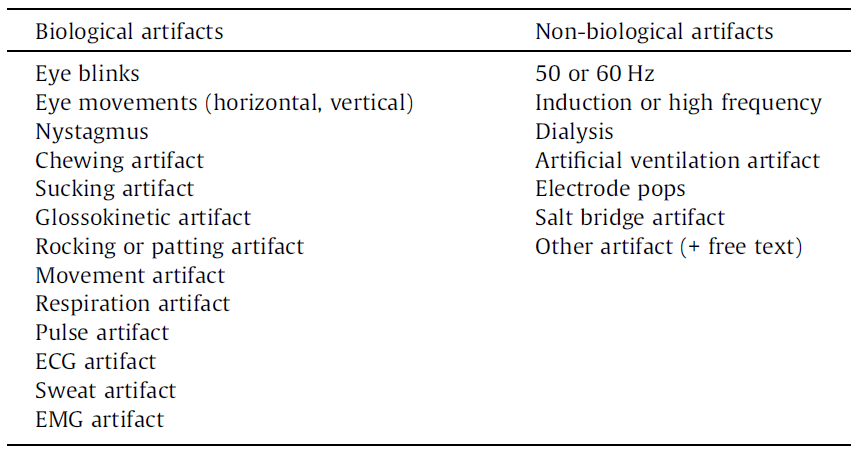
\includegraphics[width=15cm]{pic/xulun/EEGnoise.png}
	\caption{脑电信号中的噪声。}
	\label{fig6}
\end{figure}

目前伪迹去除的方式主要有三种:1. 对于小样本脑电数据,电生理专家或者临床医生根据经验浏览脑电波识别伪差;目前,对靠视觉识别伪差的可参考的标准有国际临床电生理联盟推出的SCORE\citing{beniczky2017standardized}和James Rowan的脑电波误差手册\citing{lara2015rowan}; 2. 假设伪差与脑电信号是相互独立的,采用独立成分分析\citing{delorme2007enhanced,jung2000removing}分解脑电信号并画出每个成分权重的地形图,根据地形图的形状、偶极子拟合、功率谱曲线等经验来标注成分的类型\citing{pion2019iclabel}并拒绝伪差成分,一般通过EEGLAB\citing{delorme2004eeglab}进行;3. 具有独立成分分析同时又含有如坏道挑选、滤波、参考变换、插值、回归等功能,特别是能够对成分进行自动分类,这些方法如MARA\citing{winkler2011automatic}、FASTER\citing{nolan2010faster}、ADJUST\citing{mognon2011adjust}、SASICA\citing{chaumon2015practical}、Automagic\citing{pedroni2019automagic}等。

\subsection{谱分析}
脑电是神经源的同步放电形成的,自然脑电信号中含有覆盖一定频带范围的有节律的活动\citing{niedermeyer_electroencephalography_2005,buzsaki2006rhythms}。谱分析是定量脑电的关键内容,用以量化脑电不同频带的节律震荡。 在Berger第一份关于$\alpha$、$\beta$波的报道中,他可能相信不同的节律波反映了大脑的不同状态。如今已经有大量的研究发现脑电谱与人类行为、认知状态、精神疾病之间有显著联系。 根据不同的频带特性,脑电频带划分为$\delta$(1-3Hz)、$\theta$(4-7Hz)、$\alpha$(8-12Hz)、$\beta$(15-30Hz)和$\gamma$(31-100Hz)。尽管脑电频带的划分不尽相同,但定义频带小于1Hz的微小差异不会有太大影响\citing{nuwer1999ifcn}。一般低频带反映了潜意识的状态,主要在深度睡眠和困倦时具有占优活动,高频带主要和更加警醒、活跃或与更高级认知功能相关的状态\citing{jensen2007human,sanei2013eeg}。

谱分析的必要步骤是首先通过傅里叶变换将脑电的时间序列信号从时域的幅度变化转换为频域单位时间内震荡的次数,再通过谱估计得到对应每个频率下的能量\citing{kay1999modern,stoica2005spectral}。谱分析的方法包括非参数估计例如周期图法、Welch法、Multitaper法等和参数估计如自回归模型等。 谱分析后,我们一般按照频带分析每个频带的绝对谱能量、相对谱能量和谱的地形图分布\citing{Li2019eeg}。 定量脑电中,我们将谱的特征与数据库的谱常模进行对比,研究被试与正常值的偏差\citing{Kim2018}。

除了多通道电极的功率谱分析,还可以分析电极之间的交叉谱和双谱、三阶谱等\citing{nikias1993signal}。 其中,交叉谱分析是进行头表或神经源之间频域连接、网络分析的常见步骤。

\subsection{回归}
作为统计模型的一种,回归分析用以揭示数据中一个或多个自变量与因变量之间的关系,也可用于预测和推断因果关系。使用回归方法进行预测包含数据集变量值以内的插值(内插)和变量值以外的插值(外推)。常见的回归模型包括线性回归、多项式回归、广义线性模型、逻辑回归、具有固定效应和随机效应的混合模型、非线性回归、非参数回归、鲁棒回归、局部移动回归等。

其中线性回归是最简单的形式,采用普通的最小二乘法找到唯一的曲线或超平面使得拟合数据与实际数据之间差的平方和最小。

混合模型中当自变量参数被认为是固定非随机的这种自变量被称为固定效应,当自变量参数被认为来自于群体随着个体而变化这种自变量被成为随机效应\citing{pinheiro2006mixed,demidenko2013mixed}。固体效应和随机效应并没有严格的定义和区分,在实际的不同应用中
有所不同\citing{gardiner2009fixed}。在生物学统计分析中,固定效应代表了与整个被试群体的平均有关的因素而随机效应代表了
与被试个体有关或者未知的难以控制的因素\citing{laird1982random}。我们也可以认为如果个体的潜在未观测的异质性与自变量无关就
可以视为随机效应,反之则为固定效应。 一种常用的表示混合效应模型的自变量阶数交互作用与因变量之间关系的是Wilkinson符号\citing{wilkinson1973symbolic},利用这种符号方便表示去除某个自变量或者交互项。

非参数回归是对没有固定形式的自变量的一类回归,通常需要较大的样本量,例如高斯过程回归(Kriging)和核回归。 其中高斯过程回归利
用基于先验协方差的高斯过程进行插值,常用于空间分析中考虑对一个随机空间场的个别点的估计,是一种重要的空间插值方法。从贝叶斯的角度,空间中不同点的函数估计服从高斯过程的协方差先验\citing{williams1998prediction}。在空间中对某点的估计可以通过计算该点周围已知点的加权平均,基于协方差先验,这种方法被证明是最优线性无偏估计量。这种高斯过程回归可以理解为具有协方差再生核的希尔伯特空间插值\citing{wahba1990spline}。 

局部移动回归\citing{garimella2017simple,cleveland1988locally}是局部多项式回归和移动平均的推广,常见的两种方法有局部估计
的散点图平滑(Local Estimation Scatterplot Smoothing, LOESS)和局部加权的散点图平滑\citing{cleveland1981lowess}(Local Weighted Scatterplot Smoothing, LOWESS)。

对于回归模型参数的估计,常见的方法有最小二乘、脊回归(或Tikhonov正则化)、贝叶斯线性回归、迭代再加权最小二乘等。

\subsection{震荡节律分析}
人们通常认为脑电信号中的节律是由丘脑皮层系统中的大范围抑制过程的神经同步活动引起\citing{andersen1968physiological,Steriade1990},或者兴奋抑制神经元之间的负反馈形成\citing{freeman1975mass},也可能依赖于感兴趣的频带来自于上述二者。震荡节律分析是通过提取谱的特征进行的。 傅里叶变换将脑电波分解为频率和幅度不同的正弦曲线,谱分析使我们能够得到反映震荡的不同周期性(节律)信息,某个频带的有节律的周期震荡信息表现为谱峰。大量研究表明周期震荡和生理、认知、行为、疾病状态有关。同时大脑中也存在随年龄、认知状态、任务压力改变和生理过程有关的非周期震荡。与周期震荡有关的特征是代表共振频率的谱峰在频率上位置、代表震荡强度的谱峰的能量、代表震荡频率范围的谱峰的带宽等。在脑电谱曲线中,代表周期震荡的有节律活动的谱总是与非周期震荡的活动的谱叠加在一起。非周期的震荡信息在谱中表现为随着频率增加而下降的曲线,这条曲线被称为1/f过程或者粉噪声(pink noise)。非周期震荡谱的斜率与神经源群的兴奋抑制的共济效应有关\citing{gao2017inferring},非周期震荡谱的截距可能与整个神经源群的集体放电\citing{manning2009broadband,miller2012human}、fMRI的BOLD信号有关\citing{winawer2013asynchronous}。

\section{定量脑电}
1932年,\cite{Dietsch1932}Dietsch首次使用傅里叶变换分析七例头表脑电,这是定量脑电的开始\citing{Kaiser2005}。
19世纪80年代,美国纽约大学脑研究实验室的E. R. John在\cite{john1977neurometrics,john1980developmental}提出了定量脑电的概念。定量脑电是基于静息态脑电谱常模的诊断方法,这种谱常模可由正常脑电谱特征进行z变换调整关于年龄因素的均值和偏差得到。z变换如\eqref{z变换}所示,
\begin{equation*}\label{z变换}
z=\frac{x-\mu}{\sigma}
\end{equation*}
这里的$x$可以是关于任意脑电谱特征,$\mu$和$\sigma$分别是该特征关于被试群体年龄因素的均值和标准偏差。
在定量脑电常模估计的基础上,定量脑电的诊断方法还包括定量频谱特征分析和预测诊断等等。定量脑电在神经反馈和临床诊断的应用可以参考\cite{budzynski2009introduction,simkin2014quantitative}。

定量脑电分析是相对于视觉分析脑电波的波形特点如节律的快慢、纺锤波的有无、痫样放电的出现等这样的定性分析而言的。 定性分析容易受到经验和专业知识的影响,这就促进了人们使用更加客观的定量分析方法。本论文中的定量脑电特指传统意义上基于静息态脑电谱特征面向诊断应用的方法,相似的描述也表述在\cite{kropotov2010quantitative,evans1999introduction,nuwer1988quantitative}中。更加广义来讲,采用数学和统计学分析方法能够描述那些用视觉难以描述的特征就属于定量脑电分析,有学者给出了更广义的定量脑电分析方法描述,感兴趣的读者可以参考\cite{tong2009quantitative,majumdar2017brief}。

\section{当前定量脑电方法存在的问题}
随着高性能计算、统计学习方法的进展,当前的定量脑电分析存在的一些问题可能取得如下进展: 1.多样的数据格式有待统一到BIDS标准\citing{pernet2019eeg},便于数据的分享;2.脑电的参考选择问题,多种的参考方法需要标准化起来,减少数据之间因为参考带来的差异,便于数据之间的存储和实验室间的比较研究;3.当前的脑电数据伪差去除主要是基于独立成分分析的方法,缺乏进行质量控制的标准,对于定量脑电来说,缺乏一种对谱数据进行质量控制的准则;4.存在某个地区的脑电谱常模,我们还不清楚能否建立多国家之间或者国家通用的脑电谱常模,建立一种国际通用的脑电谱常模便于进行大样本数据分析得到更加信服的结果并用于国际上某个地区特殊群体的疾病诊断;5. 当前只存在对谱曲线中$\alpha$节律成分和背景神经震荡的基于t型曲线或者高斯核函数的拟合,还不存在一种有效的提取常模数据谱节律成
分及其特征的方法;6. 当前的谱常模是基于功率谱的单变量分析,并没有考虑神经源之间的连接,有待从单变量功率谱扩展到多变量交叉谱
或者相干网络; 7. 当前基于功率谱常模的特征提取、分类诊断都是在欧式空间,我们可以借助于黎曼学习直接对交叉谱矩阵在黎曼流形上进行分析,采用更加符合数据空间特性的方法可能会找到更加准确的生物标记物。 这些问题及可能取得的进展如图\ref{qEEGnext}所示。
\begin{figure}
	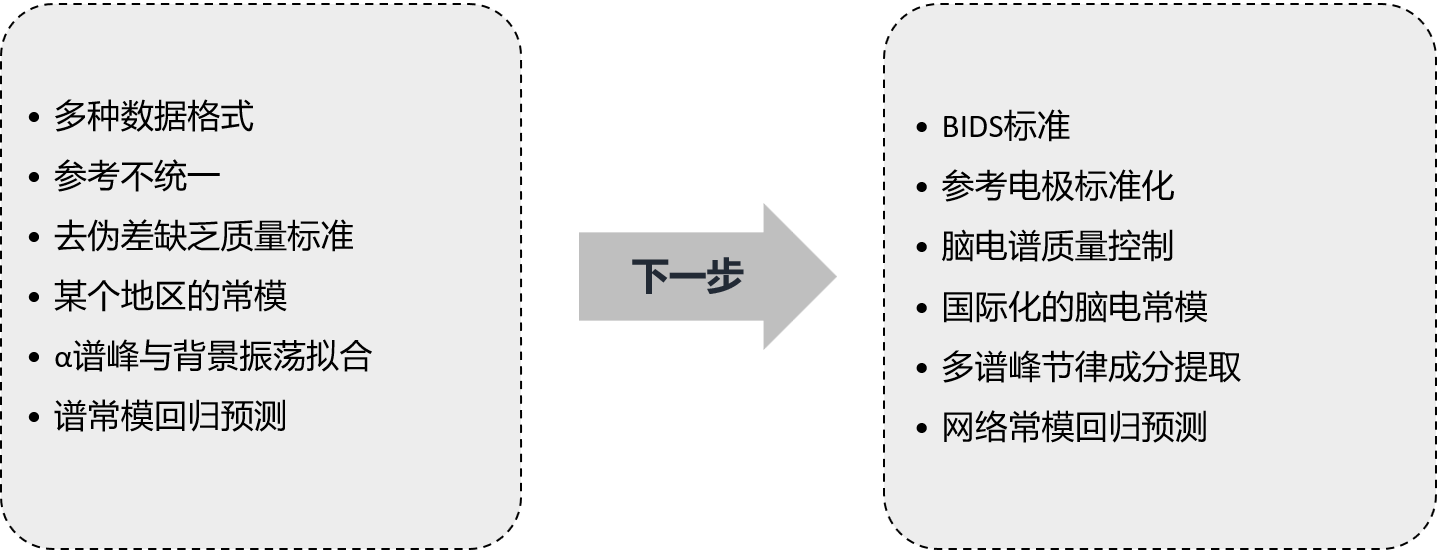
\includegraphics[width=10cm]{pic/xulun/qEEGnext.png}
	\caption{当前和下一代定量脑电方法进展}
	\label{qEEGnext}
\end{figure}

因为定量脑电是基于静息态谱常模特征的诊断方法,我们把影响谱估计和应用的方法看作最亟待解决的问题。 已经有不少文献发现脑电参考的选择对谱分析具有重要影响,如\cite{nunez_p_l_eeg_1997}指出参考对谱和相干网络估计带来的失真,\cite{yao_d_comparative_2005}发现参考能够影响谱地形图成像,\cite{chella_f_non-linear_2017}发现参考对脑电双谱分析带来的失真等,以及\cite{thatcher2004eeg}认为参考会引起相位滞后指数之间的差异等。当前,两个广泛使用的参考是平均参考\citing{offner_eeg_1950}和参考电极标准化技术(又称为零参考REST)\citing{yao_method_2001}。二者基于不同的假设,它们在实际应用中的差异并不清楚,不同的研究团队可能根据自己
的喜好选择使用。与参考问题相似,影响谱分析的是如何对大量脑电数据的去伪差程度或者谱的质量进行控制,避免在大量数据分析中包含有高度同构的谱数据,对常模的估计造成干扰。
\section{本文拟解决的问题}
本文中,我们首先对定量脑电谱分析具有根基性作用的参考问题和谱质量准则入手,研究在实际数据采集的不同因素下,参考对逼近无穷远参考下脑电电位的效果,探究参考对不同物理因素的鲁棒性;其次,我们希望利用统计学习的方法找到参考选择的基于模型选择的证据;然后,我们将分析不同参考之间的关系,平均参考和零参考物理假设的数学意义;我们希望找到能够对大样本脑电数据的谱质量进行初步筛选的准则。
在此基础上围绕定量脑电谱常模的估计以及更高阶的应用,我们希望探讨不同国家或被试群体之间是否存在一致的脑电谱常模演化曲线的问题试图对多国家脑电数据估计出谱常模,最后找到分离谱节律成分的一种合理方法并在公开数据集上得到初步应用。

\section{本文的主要贡献与创新}
本论文以定量脑电中的参考问题、谱数据质量控制、多国家脑电谱常模构建和谱节律成分的分离提取为重点研究内容,主要创新点与贡献如下:

1. 从参考的物理学假设出发,我们首次全面系统综合地分析了参考模态和电极配置等多种因素对脑电电位准确性的影响,这些因素包括:从稀疏到致密的11种覆盖我们从临床到科研所能见到的电极数目、2种电极分布即头表按距离等分的分布如10-20/10/05标准和按照多边形剖分的测地网GSN标准、不同的头模型(三层同心球头模型和借助于解构磁共振数据建立的真实头模型)、零参考中容积传导模型相对于实际的扰动、神经源偶极子的位置方向、头表电极的位置以及电极噪声等。 我们的主要贡献是发现平均参考并不随电极数目的增多而改善,对其更加重要的是电极覆盖区域,以及平均参考在竖直的偶极子径向于皮层活动时具有较大的误差,对容积传导模型的扰动和准确性没有改变零参考相对于平均参考的优势,与我们一直以来对这两种参考基于物理学假设直观的认识不同,这些结果使我们对二者对物理因素的效果差异有了新的认识。

2. 与基于电位误差大小进行参考选择不同,我们首次提出了广义线性参考模型,利用惩罚的最大似然估计发现平均参考和零参考服从参考的通解,二者的区别在于先验的协方差的差异,最后利用广义交叉验证、Akaike和Bayesian信息准则对二者基于仿真和实际数据进行选择,我们发现零参考具有比平均参考更优的模型。 我们还首次发现广义交叉验证是实际零参考应用中选择去噪参数的最优准则,提出了在实际的零参考应用中可采用被试群体的平均传递矩阵来代替被试个体传递矩阵。 主要贡献是我们首次提出了基于贝叶斯的统一的参考统计学架构,认为平均参考是基于多通道脑电信号之间相互独立的假设而零参考是基于容积传导模型的先验假设,第一次从贝叶斯和模型选择的角度发现了零参考优于平均参考。

3. 我们研究了更多种情况的单极参考,发现了它们具有满秩减一的特性。 将该特性推广到无穷远参考下的传递矩阵上并通过满秩减一型矩阵逆引理,我们首次证明零参考和平均参考、连接耳参考以及其他在线记录参考一样都是单极参考。 基于零参考和平均参考的物理学假设,我们首次从约束的线性回归解的角度推导出了零参考和平均参考,证明了二者是在对应约束下的合理选择。 我们建立了单极参考家族,分析了单极参考具有三个显著的属性,分别是无记忆性,即单极参考之间相互独立可以任意变换,单极参考都具有满秩减一的属性,和单极参考算子和单极参考下传递矩阵的正交投影分别具有中心化(等同于平均参考)和加权中心化的属性,证明了零参考与其他参考的不同在于借助于容积传导模型进行加权中心化。

4. 我们首次发现了脑电预处理过度导致的多通道谱平行或者谱同构的问题。 基于共同主成分分析,我们提出了衡量谱同构异质性的准则,用这种准则我们可以对谱质量进行初步筛选,避免构建常模中高度同构的数据。借助于三个国家基本覆盖生命周期的数据,我们使用线性混合效果模型首次研究了脑电常模构建是否依赖于国家或个体因素,最终肯定了我们的假设。这是第一个试图建立国家化通用脑电谱常模的研究。

5. 我们发现脑电谱成分拟合的合理准则是对具有独立于频率的复高斯分布的傅里叶系数进行最大Whittle似然估计,认为谱多个节律成分的分离问题是协方差丢失的不完全数据估计问题可以通过最大似然估计来求解。 我们使用信号处理峰值选择程序可以较好地定位出谱曲线中的节律成分位置,在对单个成分的拟合中,我们首次采用了平滑和形态约束以满足成分形态各异的特点。

\section{本论文的结构安排}
本文的章节结构安排如下:
\begin{description}
	\item[第一章] 绪论。
	\item[第二章] 以参考模态和电极配置为重点研究定量脑电中电势对多种物理因素的影响。
	\item[第三章] 提出了脑电的广义参考模型,描述了脑电无穷远参考的统一的贝叶斯统计学架构,对平均参考和零参考进行基于统计模型指数的选择。
	\item[第四章] 证明了零参考是一种单极参考,利用平均参考和零参考的物理约束通过线性回归的方法推导除了平均参考和零参考,描述了单点参考的统计学属性以。
	\item[第五章] 描述了大样本脑电谱的同构性基于的筛选准则,并在三个样本大小不同的数据集上进行测试。以及多国家脑电谱常模的研究。
    \item[第六章] 发展了基于Whittle似然和非参数估计的谱节律成分提取算法,并应用在公开的颅内数据集中,通过特征提取,我们得到了谱特征地形图。
	\item[第七章] 总结与展望。
\end{description}
